\documentclass{article}
\setlength{\parskip}{5pt} % esp. entre parrafos
\setlength{\parindent}{0pt} % esp. al inicio de un parrafo
\usepackage{listings} % listings
\usepackage{color} %colores
\usepackage{amsmath} % mates
\usepackage[sort&compress,numbers]{natbib} % referencias
\usepackage{url} % que las URLs se vean lindos
\usepackage[top=15mm,left=20mm,right=20mm,bottom=25mm]{geometry} % margenes 
\usepackage{hyperref} % ligas de URLs
\usepackage{graphicx} % poner figuras
\usepackage[spanish]{babel} % otros idiomas


\author{Claudia Lizeth Hern\'andez Ram\'irez} % author
\title{Homework 9 - Interacciones entre part\'iculas} % titulo
\date{\today}

\definecolor{mypurple}{rgb}{0.305, 0.066, 0.592}
\definecolor{mygray}{rgb}{0.976, 0.980, 0.980}
\definecolor{myorange}{rgb}{0.933, 0.305, 0.090}
\lstset{ 
  backgroundcolor=\color{mygray},
  commentstyle=\color{myorange},
  keywordstyle=\color{mypurple}, 
  numberstyle=\tiny\color{myorange}
  stringstyle=\color{mypurple}, 
  breaklines=true,
}


\begin{document} % inicia contenido

\maketitle % cabecera



% INTRODUCCIOOOOOOOOOOOON
\section{Introducci\'{o}n}\label{intro} % seccion y etiqueta
Agregar a cada part\'icula una masa y hacer que esa masa cause fuerzas gravitacionales (atracciones) adem\'as de las fuerzas causadas por las cargas. Estudiar la distribuci\'on de velocidades de las part\'iculas y verificar gr\'aficamente que est\'e presente una relaci\'on entre los tres factores: la velocidad, la magnitud de la carga, y la masa de las part\'iculas. Tomando en cuenta que la velocidad tambi\'en es afectada por las posiciones.


% DESARROLLOOOOOOOOOOOO
\section{Desarrollo}\label{desarrollo} % Desarrollo de la tarea

Comenc\'e trabajando con el c\'odigo que se nos explic\'o en clase \cite{Cbase}. Posteriormente, agregu\'e la masa a mi programa, siendo esta un valor aleatorio y normalizado.

Trabaj\'e con 25 part\'iculas, 55 iteraciones y 10 repeticiones.

\begin{lstlisting}[language=R, caption= Segmento de c\'odigo se agrega la masa.]

n <- 25 #cantidad de particulas
datos = data.frame()
repeticiones = 1:10

for (reply in repeticiones) {
  p <- data.frame(reply, x = rnorm(n), y=rnorm(n), c=rnorm(n), m=rnorm(n))
[...]
    mmax = max(p$m)
    mmin = min(p$m)
    p$m = (p$m - mmin) / (mmax - mmin) + 0.001
\end{lstlisting}

De igual forma, se modific\'o la parte que afecta la masa a la funci\'on.

\begin{lstlisting}[language=R, caption= Segmento de c\'odigo funci\'on-masa.]

fuerza <- function(i) { #datos de la particula i
  xi <- p[i,]$x
  yi <- p[i,]$y
  ci <- p[i,]$c
  mi = p [i,]$m #masa
  G = 0.6674 #Valor ficticio de Constante de Gravitacion Universal
  
  fx1 = 0
  fy1 = 0
  fx2 = 0
  fy2 = 0
  for (j in 1:n) {
    cj <- p[j,]$c
    mj = p[j,]$m
    dir <- (-1)^(1 + 1 * (ci * cj < 0))
    dx <- xi - p[j,]$x
    dy <- yi - p[j,]$y
    factor <- dir * abs(ci - cj) / (sqrt(dx^2 + dy^2) + eps) #carga entre particulas
      factor1 <- G * ((mi * mj) / ((sqrt(dx^2 + dy^2) + eps)^2)) #masa entre particulas
    
    fx1 = fx1 - dx * factor
    fy1 = fy1 - dy * factor
    fx2 = fx2 - dx * factor1
    fy2 = fy2 - dy * factor1
    
    fx = fx1 + fx2
    fy = fy1 + fy2
\end{lstlisting}

Con la formula de la \texttt{Fuerza Gravitacional}\cite{ecuaciones}:

\begin{equation}
\label{eq:FzaGravitacional}
F = G \dfrac{m_1 * m_2}{r^2}
\end{equation}
\bigskip
Se determin\'o como afectar\'ia la masa a mis part\'iculas.
\bigskip

\begin{lstlisting}[language=R, caption= Segmento de c\'odigo velocidad.]

p$vel=numeric(n)
for (iter in 1:tmax) {
  f <- foreach(i = 1:n, .combine=c) %dopar% fuerza(i)
  delta <- 0.02 / max(abs(f)) # que nadie desplace una paso muy largo
  p$x <- foreach(i = 1:n, .combine=c) %dopar% max(min(p[i,]$x + delta * f[c(TRUE, FALSE)][i], 1), 0)
  p$y <- foreach(i = 1:n, .combine=c) %dopar% max(min(p[i,]$y + delta * f[c(FALSE, TRUE)][i], 1), 0)
  v =    foreach(i = 1:n, .combine=c)%dopar% sqrt((delta * f[c(TRUE, FALSE)][i])^2 + (delta * f[c(FALSE, TRUE)][i])^2)
  p$vel=p$vel+v
\end{lstlisting}
\bigskip

Para visualizar el comportamiento de los resultados se obtuvieron las gr\'aficas \ref{Figura 2} y \ref{Figura 3}.

\begin{figure}[htb] % figura
    \centering
    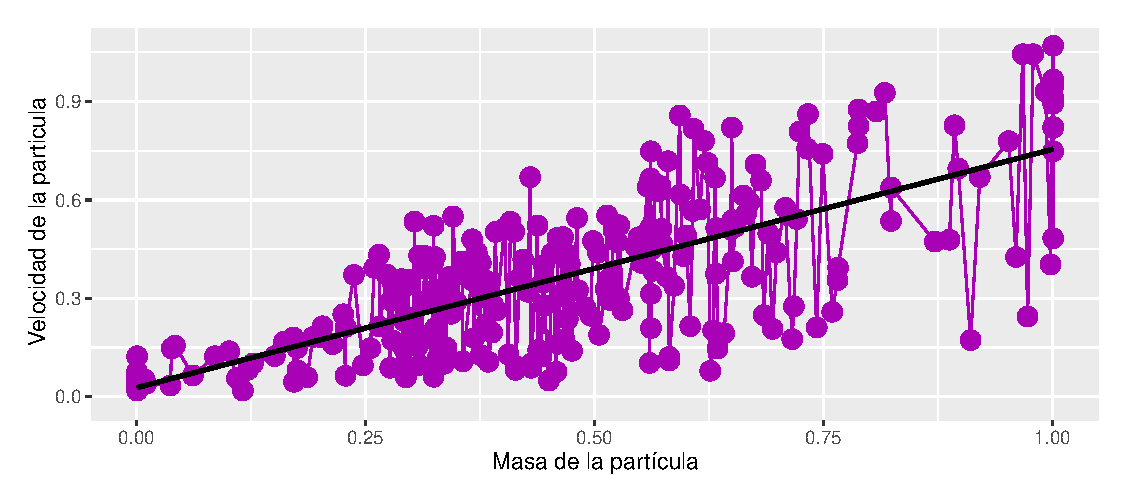
\includegraphics[width=150mm]{velvsmas.eps} % archivo
    \caption{Masa vs Velocidad.}
    \label{Figura 2}
\end{figure}
\newpage

\begin{figure}[htb] % figura
    \centering
    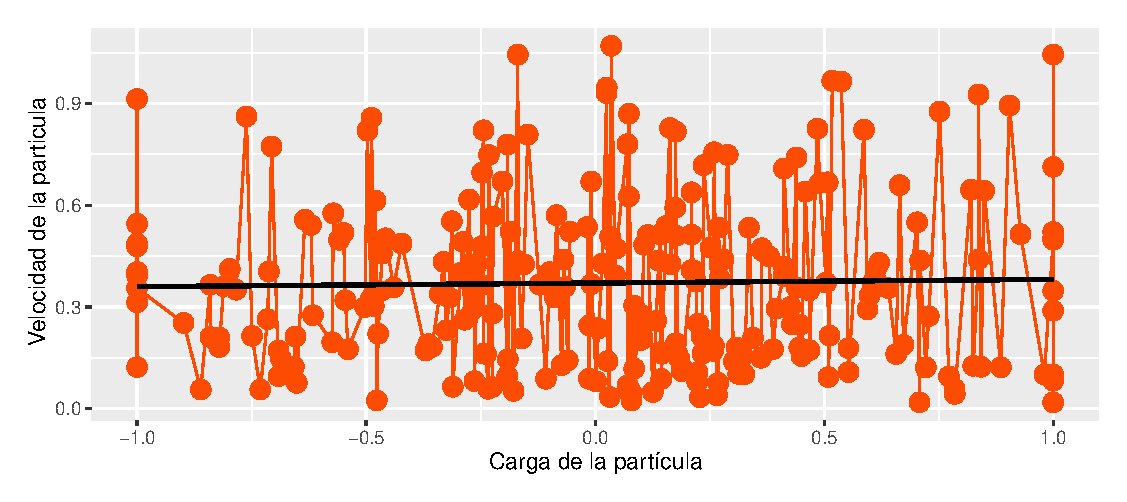
\includegraphics[width=150mm]{velvscar.eps} % archivo
    \caption{Carga vs Velocidad.}
    \label{Figura 3}
\end{figure}

\section{Estad\'istica.}

\begin{table}[ht]
    \centering
    \caption{Resultados obtenidos de prueba de normalidad de Shapiro.} 
    \begin{tabular}{|c|c|c|c|}
    \hline
    Carga & W value & P value & ¿Se acepta H0?  \\
    \hline
    -5 & 0.8914 & 0.1761 & s\'i \\
    \hline 
     -4 & 0.8561 & 0.0212 & no  \\
    \hline 
    -3 & 0.8732 & 0.0345 & no \\
    \hline 
    -2 & 0.9510 & 0.3563 & s\'i \\
    \hline
    -1 & 0.9497 & 0.1306 & s\'i \\
    \hline
    0 & 0.9241 & 0.0167 & no \\
    \hline
    1 & 0.9272 & 0.0105 & no \\
    \hline
    2 & 0.8821 & 0.0031 & no \\
    \hline
    3 & 0.8843 & 0.0308 & no \\
    \hline
    4 & 0.8669 & 0.0244 & no \\
    \hline
    5 & 0.9332 & 0.3758 & s\'i \\
    \hline
\end{tabular}
    \label{cuadro 1}
\end{table}

\begin{table}[htb]
    \centering
    \caption{Informaci\'on individual de los datos.} 
    \begin{tabular}{|c|c|c|c|c|c|c|}
    \hline
    Carga & Qty. Participantes & promedio & Desv. Std. & Varianza & Mediana & Rango Intercuartil  \\
    \hline
    -5 & 10 & 0.45 & 0.20 & 0.04 & 0.44 & 0.12 \\
    \hline
    -4 & 15 & 0.33 & 0.22 & 0.05 & 0.26 & 0.17 \\
    \hline
    -3 & 16 & 0.29 & 0.18 & 0.03 & 0.24 & 0.33 \\
    \hline
    -2 & 21 & 0.37 & 0.21 & 0.04 & 0.33 & 0.26 \\
    \hline
    -1 & 33 & 0.40 & 0.26 & 0.06 & 0.37 & 0.40 \\
    \hline
    0 & 36 & 0.37 & 0.28 & 0.08 & 0.34 & 0.38 \\
    \hline
    1 & 42 & 0.35 & 0.23 & 0.05 & 0.37 & 0.35 \\
    \hline
    2 & 30 & 0.33 & 0.21 & 0.04 & 0.27 & 0.30 \\
    \hline
    3 & 18 & 0.42 & 0.28 & 0.07 & 0.36 & 0.40 \\
    \hline
    4 & 16 & 0.34 & 0.30 & 0.09 & 0.20 & 0.45 \\
    \hline
    5 & 13 & 0.43 & 0.32 & 0.10 & 0.49 & 0.42 \\
    \hline
\end{tabular}
    \label{cuadro 2}
\end{table}
\newpage

\begin{table}[htb]
    \centering
    \caption{Diferencias entre grupos. Kruskal-Wallis.} 
    \begin{tabular}{|c|c|c|c|c|c|c|c|c|c|c|}
    \hline
    "" & -5 & -4 & -3 & -2 & -1 & 0 & 1 & 2 & 3 & 4 \\
    \hline
    -4 & 1 & "" & "" & "" & "" & "" & "" & "" & "" & "" \\
    \hline
    -3 & 1 & 1 & "" & "" & "" & "" & "" & "" & "" & "" \\
    \hline
    -2 & 1 & 1 & 1 & "" & "" & "" & "" & "" & "" & "" \\
    \hline
    -1 & 1 & 1 & 1 & 1 & "" & "" & "" & "" & "" & "" \\
    \hline
    0 & 1 & 1 & 1 & 1 & 1 & "" & "" & "" & "" & "" \\
    \hline
    1 & 1 & 1 & 1 & 1 & 1 & 1 & "" & "" & "" & "" \\
    \hline
    2 & 1 & 1 & 1 & 1 & 1 & 1 & 1 & "" & "" & "" \\
    \hline
    3 & 1 & 1 & 1 & 1 & 1 & 1 & 1 & 1 & "" & "" \\
    \hline
    4 & 1 & 1 & 1 & 1 & 1 & 1 & 1 & 1 & 1 & "" \\
    \hline
    5 & 1 & 1 & 1 & 1 & 1 & 1 & 1 & 1 & 1 & 1 \\
    \hline
\end{tabular}
    \label{cuadro 3}
\end{table}

\begin{table}[ht]
    \centering
    \caption{Resultados obtenidos de prueba Kruskal-Wallis.} 
    \begin{tabular}{|c|c|c|}
    \hline
    Chi cuadrada & DF & P  \\
    \hline
    4.9822 & 10 & 0.8924 \\
    \hline
\end{tabular}
    \label{cuadro 4}
\end{table}
\newpage


De lo anterior se muestran algunos estados obtenidos de las part\'iculas en diferentes tiempos.
\begin{figure}[h!] % figura
    \centering
    \includegraphics[width=60mm]{p9_t000.png} % archivo
    \caption{Estado inicial de las part\'iculas.}
    \label{Figura 3}
\end{figure}
\begin{figure}[h!] % figura
    \centering
    \includegraphics[width=60mm]{p9_t015.png} % archivo
    \caption{Estado de las part\'iculas en tiempo 15.}
    \label{Figura 4}
\end{figure}
\begin{figure}[h!] % figura
    \centering
    \includegraphics[width=60mm]{p9_t035.png} % archivo
    \caption{Estado de las part\'iculas en tiempo 35.}
    \label{Figura 5}
\end{figure}
\begin{figure}[htb] % figura
    \centering
    \includegraphics[width=60mm]{p9_t035.png} % archivo
    \caption{Estado de las part\'iculas en tiempo 35.}
    \label{Figura 6}
\end{figure}
\begin{figure}[h!] % figura
    \centering
    \includegraphics[width=60mm]{p9_t045.png} % archivo
    \caption{Estado de las part\'iculas en tiempo 45.}
    \label{Figura 7}
\end{figure}
\begin{figure}[h!] % figura
    \centering
    \includegraphics[width=60mm]{p9_t055.png} % archivo
    \caption{Estado de las part\'iculas en tiempo 55.}
    \label{Figura 8}
\end{figure}

\begin{figure}[htb!] % figura
    \centering
    \includegraphics[width=150mm]{Rplotcarga.eps} % archivo
    \caption{Comportamiento de la velocidad considerando carga y masa.}
    \label{Figura 9}
\end{figure}


\newpage
\section{Masas Fijas.}
Para apreciar de una mejor forma la relaci\'on que tienen las masas, se opt\'o por determinar valores fijos, en este caso masas con valores de 1, 1.5, 2, 2.5 y 3.

\begin{lstlisting}[language=R, caption= Segmento de c\'odigo - Masas Fijas.]

datos = data.frame()
masas = seq(1, 3, 0.5)
repeticiones = 1:5
n <- 25

for (masa in masas){
  for ( replica in repeticiones){
  [...]
  mmax = max(p$m) 
  mmin = min(p$m)
  p$m=masa #masa fija
\end{lstlisting}

\section{Estad\'istica de Masa Fija.}

\begin{table}[ht]
    \centering
    \caption{Resultados obtenidos de prueba de normalidad de Shapiro.} 
    \begin{tabular}{|c|c|c|c|}
    \hline
    Carga & W value & P value & ¿Se acepta H0?  \\
    \hline
    1 & 0.9671 & 0.0038 & no \\
    \hline
    1.5 & 0.8970 & $8.6\times 10^{-8}$ & no \\
    \hline
    2 & 0.9241 & $2.81\times 10^{-6}$ & no \\
    \hline
    2.5 & 0.8980 & $9.72\times 10^{-8}$ & no \\
    \hline
    3 & 0.9249 & $3.14\times 10^{-6}$ & no \\
    \hline
\end{tabular}
    \label{cuadro 1}
\end{table}

\begin{table}[ht]
    \centering
    \caption{Resultados obtenidos de prueba Kruskal-Wallis.} 
    \begin{tabular}{|c|c|c|}
    \hline
    Chi cuadrada & DF & P  \\
    \hline
    7.5389 & 4 & 0.11 \\
    \hline
\end{tabular}
    \label{cuadro 4}
\end{table}

\begin{table}[htb]
    \centering
    \caption{Diferencias entre grupos. Kruskal-Wallis.} 
    \begin{tabular}{|c|c|c|c|c|}
    \hline
    "" & 1 & 1.5 & 2 & 2.5  \\
    \hline
    1.5 & 0.468 & "" & "" & ""  \\
    \hline
    2 & 1 & 1  & "" & ""   \\
    \hline
    2.5 & 0.907 & 1 & 1 & ""   \\
    \hline
    3 & 0.085 & 1 & 1 & 1  \\
    \hline
\end{tabular}
    \label{cuadro 3}
\end{table}

\begin{figure}[htb] % figura
    \centering
    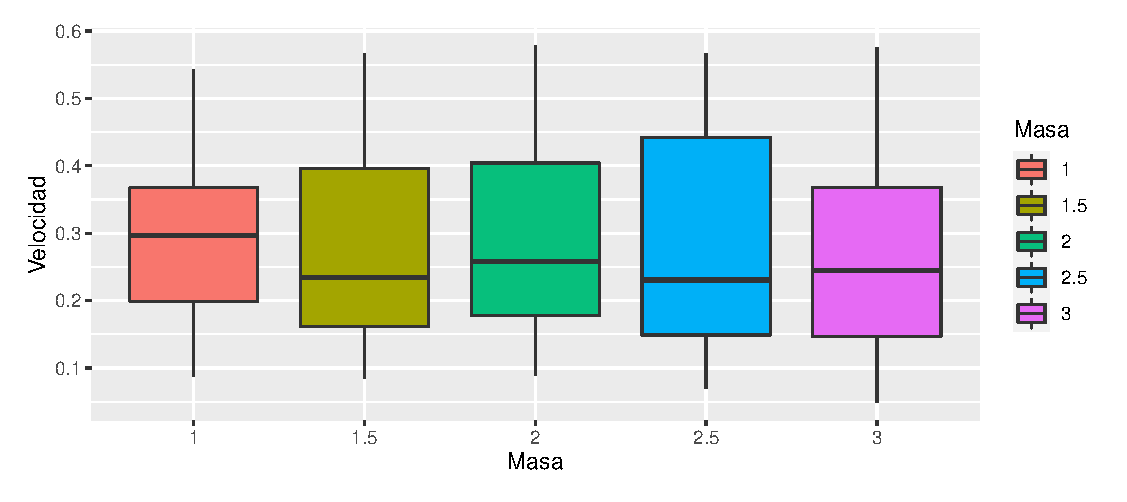
\includegraphics[width=150mm]{Rplotmasa.eps} % archivo
    \caption{comportamiento de la velocidad considerando masa fija.}
    \label{Figura 10}
\end{figure}
\newpage


%CONCLUSIOOOON
\section{Conclusi\'on.}
Se puede observar en las gr\'aficas \ref{Figura 2} y \ref{Figura 3} el comportamiento que tiene la \texttt{velocidad} con respecto a la \texttt{masa} y a la \texttt{carga} respectivamente. En la relacion con la masa podemos observar una tendencia directamente proporcional respecto a la masa, es decir, si aumenta la masa aumenta la velocidad, teniendo datos at\'ipicos. Este resultado contradice mi hip\'otesis inicial, ya que pensaba que a menor masa ser\'ia mayor la velocidad con la que se mover\'ian las part\'iculas.

Por otro lado, en la relaci\'on de la velocidad con la carga se observa una tendencia inversamente proporcional: a mayor carga, la velocidad disminuye.
por otro lado, si determinamos un valor fijo para la masa o mas estable, de igual forma, variando los valores de la carga, la velocidad no presentar\'a una diferencia significativa.

% BIBLIOGRAFIAAAAAAS
\bibliography{referencias}
\bibliographystyle{plainnat}
\end{document}


